\section{Implementation choices}
\label{sec:03-implementation}

As stated in \cref{sec:motion-models}, we decided to use an indirect method with affine model for motion estimation as in Bergen et al.\cite{Bergen92}; also, we decided to obtain a robust estimation by using a strategy similar to Dufaux and Konrad\cite{Dufeaux2000}, where they adopt a hierarchical approach to obtain a robust estimation using coarse resolution to guide the search for the best parameters at a finer resolution.

In the following sections, we will provide an in-depth explaination of our solution and present the pseudocode of the algorithm. A schematic representation of the procedure is presented in \cref{fig:implementation-flow}.

\begin{figure}
    \centering
    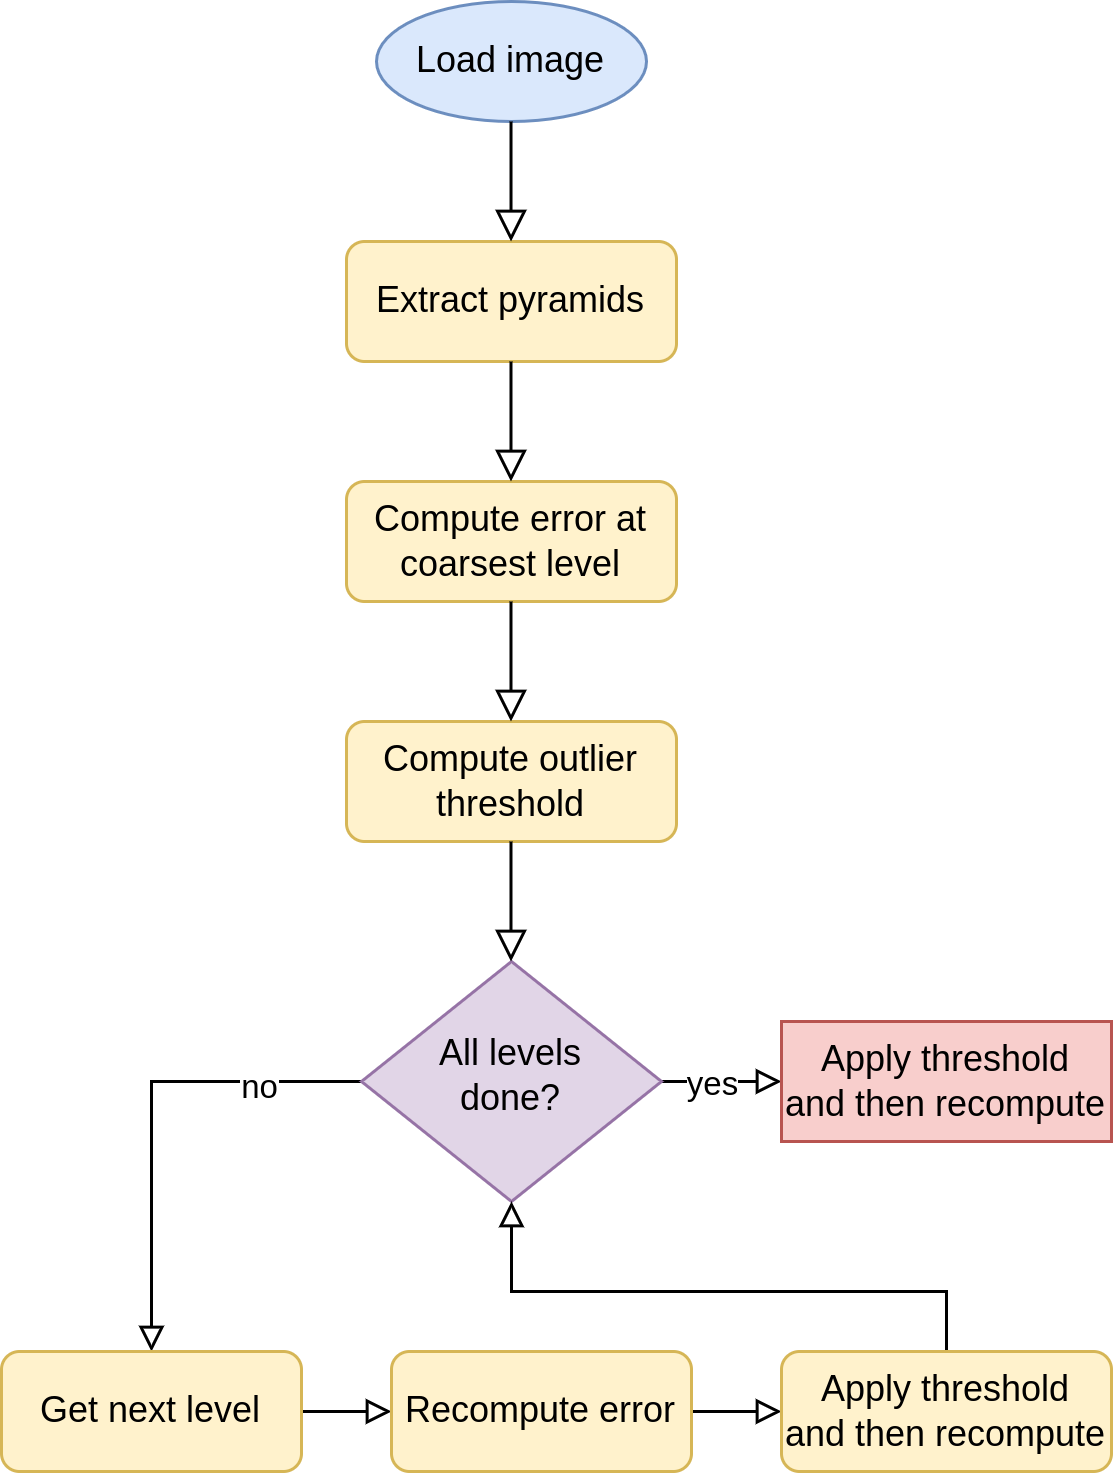
\includegraphics[width=.7\linewidth]{../assets/images/implementation-flow.png}
    \caption{Schema of the flow of implementation of the global motion estimation pipeline.}
    \label{fig:implementation-flow}
\end{figure}

\subsection{Block-Based Motion Estimation}
\label{sec:BBME}
The first piece of the architecture is the algorithm to compute the motion field to be used as ground truth.
In our case, we decided to implement a block matching motion estimation (BBME), as computing the motion field on blocks, rather than single pixels, can be much less computationally expensive.

The main idea of BBME is to divide the frame in blocks, and search for each block in the previous frame the corresponding block in the next frame.
This gives us the displacement of the block between the two frames, which is accounted as motion vector of the block.
This is the basic principle of BBME, from which derived a number of implementations that present differences mainly in two aspects:
\begin{enumerate}
    \item the size and shape of the block;
    \item the path that the searching procedure follows.
\end{enumerate}

During the project we implemented a number of these techniques:
\begin{itemize}
    \item exhaustive search;
    \item two-dimensional logarithmic search;
    \item new three-step search, from \cite{Li94};
    \item diamond search, from \cite{Zhu2000};
\end{itemize}

In the final implementation, the block matching method used is the one presented in \cite{Zhu2000}, known as diamond search (DS),  with a mean square error measure to compute (dis-)similarity between blocks.
Nonetheless, all the other methods are still present and by slightly changing the code they can be tested as well.

Here we briefly discuss the algorithm that we choose to implement and propose a small example for clarification.
The DS algorithm uses a peculiar diamond-shaped search pattern, which defines which positions will be used as target points where to center the block in the next frame to see if it corresponds to the block in the previous frame. In particular, the algorithm uses two slighlty different shapes depending on the current iteration (see \cref*{fig:ds-search-patterns}):
\begin{itemize}
    \item large diamond search pattern;
    \item small diamond search pattern.
\end{itemize}

\begin{figure}
    \centering
    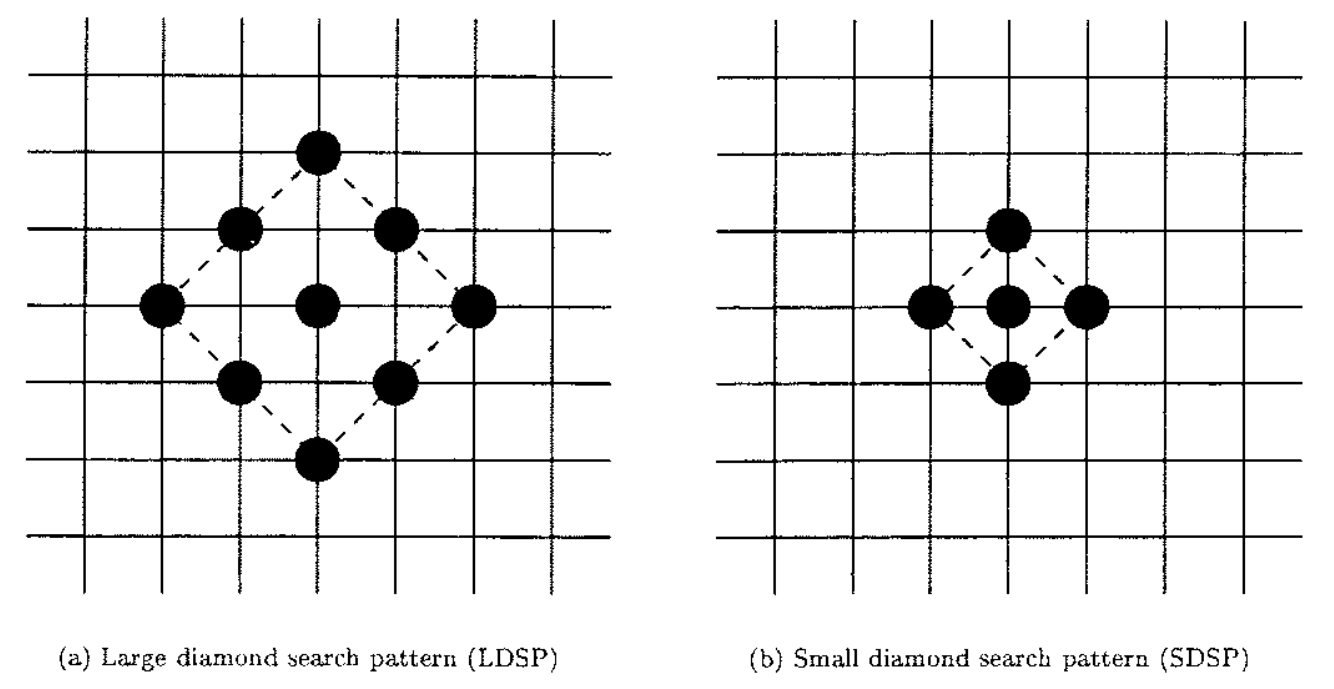
\includegraphics[width=.95\linewidth]{../assets/images/ds-search-patterns.png}
    \caption{Representation of the two DS algorithm search patterns}
    \label{fig:ds-search-patterns}
\end{figure}

The procedure is the following:
\begin{enumerate}
    \item the search starts with LDSP, meaning that we check the blocks centered in each one of the 9 positions; if the best match is the central position then we pass to the second step, otherwise we move to the best match position and re-use the LDSP;
    \item in the second step we use SDSP and look again for the best matching position among the 5 available, then return the best match position.
\end{enumerate}

\begin{figure}
    \centering
    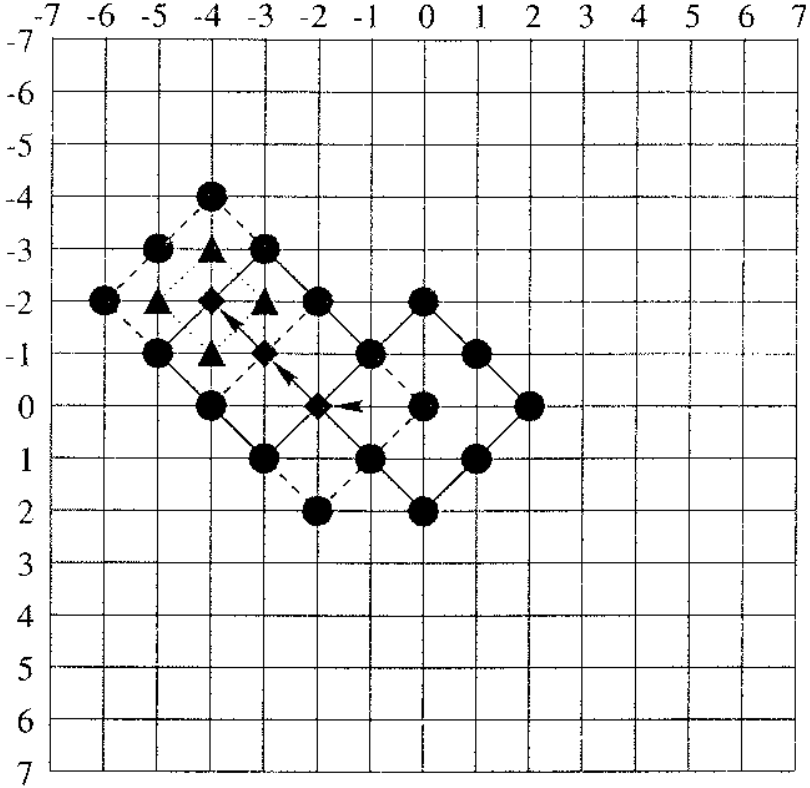
\includegraphics[width=.95\linewidth]{../assets/images/ds-exe.png}
    \caption{Example of run of diamond search algorithm for block matching motion estimation.}
    \label{fig:diamond-search-example}
\end{figure}

In \cref{fig:diamond-search-example} we can see an example of run. We can spot the three large-shape diamonds (the contour position are marked with circles) and the small shaped diamond (contour positions marked with triangles).
In this example the block matching algorithm started from $\{0,0\}$, then moved with the large diamond to $\{-2,0\}$, because this was the position that minimized the error between the block in the previous and the next frame. Then again with the large diamond the algorithm reached $\{-3,-1\}$ first, and $\{-4,-2\}$ after. Here the best matching position for the large diamond shape was $\{-4,-2\}$, therefore the algorithm stopped using the large diamond and started with the small diamond. Finally, the small diamond returned once again as best match position $\{-4,-2\}$, which was then returned as final matching position for the block in the previous frame.

\subsection{Affine Model Parameter Estimation}
In \cref{sec:motion-models}, we presented the affine motion model, which is the one we decided to use in our implementation.

To get the motion vector of a certain position $p=\{x,y\}$ in the previous frame, we can solve the following formulation of the affine model:
\begin{equation}
    \label{eq:displacement-matrix-formulation}
    d(p, a) = A(p)\;a
\end{equation}
where $d(p, a)$ is the displacement for the position $p = \{x,y\}$, given the parameter vector $a$; $A[p]$ is an intermediate matrix that is computed as 
\begin{equation*}
    \label{eq:affine-model-parameter-matrix}
    A(p) = \begin{bmatrix}
        1 & x & y & 0 & 0 & 0 \\
        0 & 0 & 0 & 1 & x & y
    \end{bmatrix}
\end{equation*}

By encoding the estimation of the motion field in this way, the $p$-norm error we are trying to minimize (see \cref{eq:indirect-estimation}), gets rewritten in this way:

\begin{equation}
    \label{eq:pnorm-error}
    E = \sum_p{\left| d(p, a) - d(p) \right|^P}
\end{equation}
Here we introduce $d(p)$ as the ground truth motion vector (the one we get from the BBME as in \cref{sec:BBME}) and $P$ which specifies the grade of the $p$-norm used. In this case we decided to set $P=2$, following the procedure explained in \cite{WangBook}. Pay attention to the difference, in the formula, between $p$ (the position) and $P$ (the grade of the $p$-norm). 

The next step is to minimize the error in \cref{eq:pnorm-error} with respect to the parameter vector $a$.
The procedure in \cite{WangBook} states that we need to compute the gradient of $E$ w.r.t $p$, and then get the value of $a$ that sets the gradient to 0.

By using the matrix formulation explained in \cref{eq:displacement-matrix-formulation} and by setting the gradient $\nabla_a E = 0$, we obtain the following result:
\begin{equation}
    \label{eq:optimal-parameter-affine}
    a = \left (\sum_p A[p]^T A[p] \right )^{-1} \left (\sum_p A[p]^T d(x) \right)
\end{equation}

There are three interesting notes about \cref{eq:optimal-parameter-affine}:
\begin{enumerate}
    \item we are iterating over a set of positions $p$: it's interesting to notice that these points do not need to cover the complete scene, i.e. we can use only a subset of the image to optimize the parameters;
    \item each one of the points can be weighted with a weight $w(p)$ as shown in \cref{eq:optimal-parameter-affine-weighted};
    \item we can actually split the computation of the parameter vector $a = [a_1, a_2, a_3, b_1, b_2, b_3]$ in two different slices, $a_x = [a_1, a_2, a_3]$ and $a_y = [b_1, b_2, b_3]$, which can be computed in a specular way as shown in \cref{eq:optimal-parameter-affine-weighted-halved} this is useful to further reduce the complexity of the procedure.
\end{enumerate} 

\small
\begin{equation}
    \label{eq:optimal-parameter-affine-weighted}
    a = \left (\sum_p w(p) A[p]^T A[p] \right )^{-1} \left (\sum_p w(p) A[p]^T d(x) \right)
\end{equation}
\begin{equation}
    \footnotesize
    \label{eq:optimal-parameter-affine-weighted-halved}
    a_x = \left (\sum_p w(p) A_x[p]^T A_x[p] \right )^{-1} \left (\sum_p w(p) A_x[p]^T d_x(x) \right)
\end{equation}
where $A_x(p) = [1,x,y]$.

The form of the solution that we used in the implementation is the one reported in \cref{eq:optimal-parameter-affine-weighted-halved}.

\subsection{Hierarchical Robust Estimation}

The last part of the project is a strategy used to provide a robust estimation of the parameters for the affine motion model.
The proposed implementation is inspired by \cite{Dufeaux2000}, where the computation of the motion field takes place at different levels of resolution subsequently.

The main idea is to compute the parameter vector $a$ at a coarser resolution, and then use this coarser estimation to extract information useful for regularizing the estimation at finer resolutions. 
In practice, this translates in our code being structured as shown in \cref{fig:implementation-flow}: the two frames we use as previous and next frame are, first of all, transformed in multi-resolution pyramids, and then used iteratively for the process of parameter estimation.

Here we report a summary of the procedure used to implement the hierarchical robust etimation:
\begin{enumerate}
    \item for each iteration we get as input the frames at the corresponding level $l$ of the pyramid (at a finer resolution w.r.t the previous iteration at level $l-1$) and the parameter vector $a_{l-1}$ computed in the previous iteration;
    \item we use the (scaled) parameters $a_{l-1}$ to compute the error for each position $p$ in the frames at level $l$; error is computed as difference between the ground truth motion vector in $p$ and the motion vector obtained with the motion model in $p$ with parameters $a_{l-1}$;
    \item to detect the outliers we order all positions $p$ by the magnitude of the error, we set a fixed percentage \texttt{outlier\_percentage} and all the positions that fall in that percentage of higer-error-positions are marked as outliers;
    \item once we have marked all the outliers, we can proceed and compute the new estimate of the parameter vector $a_{l}$ ignoring the outliers;
    \item the new estimate will be returned to the next level $l+1$ of the hierarchical procedure, or simply returned to the caller of the function when we reach the last level.
\end{enumerate}

\begin{algorithm}[H]
    \DontPrintSemicolon
    
    \SetKwData{params}{\(a\)}
    \SetKwData{out}{outliers}
    \SetKwData{prevp}{prev\_pyrs}
    \SetKwData{curp}{cur\_pyrs}
    \SetKwData{prevf}{prev\_frame}
    \SetKwData{curf}{cur\_frame}
    \SetKwData{gt}{ground\_truth\_mfield}
    \SetKwData{est}{estimated\_mfield}
    
    \SetKwFunction{Pyr}{get\_pyr}
    \SetKwFunction{FirstEst}{first\_estimation}
    \SetKwFunction{Next}{next}
    \SetKwFunction{BM}{BBME}
    \SetKwFunction{Aff}{affine}
    \SetKwFunction{DetOut}{detect\_outliers}
    \SetKwFunction{Min}{minimize\_error}
    
    \KwIn{\textit{previous\_frame}, \textit{current\_frame}}
    \KwOut{\params \quad \texttt{//\(\;\)parameter vector}}
    \;        
    \prevp = \Pyr{previous\_frame}\;
    \curp = \Pyr{current\_frame}\;
    \params = \FirstEst{\prevp.\Next{}, \curp.\Next{}}\;
    \ForEach{\(l\) in levels}{
        \prevf = \prevp.\Next{}\;
        \curf = \curp.\Next{}\;
        \gt = \BM{\prevf, \curf}\;
        \est = \Aff{\params}\;
        \out = \DetOut{\gt, \est}\;
        \params = \Min{\prevf, \curf, \out}\;
        }
        
        \Return \params\;
        
        \caption{High-level pseudocode of our solution.}
        \label{alg:gme}
    \end{algorithm}


% prev_pyr = get_pyr(previous_frame)
% curr_pyr = get_pyr(current_frame)
% a = first_estimation(prev_pyr.pop(), curr_pyr.pop())
% for level in ([1,2]):
% 	curr = curr_pyr.pop()
% 	prev = prev_pyr.pop()
% 	ground_truth_mfield = BMME_motion_estimation(prev, curr)
% 	estimated_mfield = affine(a)
% 	outliers = detect_outliers(ground_truth_mfield, estimated_mfield)
% 	a = minimize_error(prev, curr, outliers)# update parameters
% return a